\documentclass[12pt]{article}

\usepackage{amsmath,amsthm}
\usepackage{amsfonts}
\usepackage[psamsfonts]{amssymb}
\usepackage{palatino,euler} 
\usepackage[applemac]{inputenc}
\usepackage[french]{babel}
\usepackage[T1]{fontenc}
\usepackage{graphicx}
% \usepackage{tikz}
\usepackage{hyperref}


\setlength{\topmargin}{0pt}
\setlength{\headheight}{0pt}
\setlength{\headsep}{0pt}
\setlength{\textheight}{612pt}
\setlength{\textwidth}{400pt}
\setlength{\marginparwidth}{0pt}
\setlength{\oddsidemargin}{36pt}
\setlength{\parskip}{\baselineskip}
% \setlength{\parindent}{0pt}

\newcommand\rn[1]{\romannumeral #1}


\title{MAT1460\\[3ex]L'\'epid\'emie d'influenza 2017-2018 demeure-t-elle dangereuse?}
\author{Pelletier, Xavier\\[1ex] Chen, Siying\\[1ex]L\'evesque, \'Etienne\\[1ex] Grenier, David}
\date{}
\begin{document}

    \maketitle
    \thispagestyle{empty}
    \vfill
    \begin{center}
    Universit\'e de Montr\'eal

    \today
    \end{center}
    \clearpage

    \section{Introduction}

L'\'epid\'emie annuelle d'influenza occasionne un impact important pour la soci\'et\'e; il serait
donc important de pouvoir \'evaluer la situation au cours d'une saison donn\'ee. On cherche donc \`a
mesurer la dangerosit\'e \`a partir des donn\'ees disponibles.

Nous pr\'esentons un mod\`ele permettant d'\'evaluer le niveau de dangerosit\'e \`a partir des
donn\'ees g\'en\'eralement fournies par divers organismes\cite{InfluenzaQC}, soit, le nombre de
tests d'influenza effectu\'es chaque semaine ainsi que le nombre de ceux qui sont positifs. L'impact
de l'influenza est mesurable en terme de vies perdues, de frais m\'edicaux et d'impact
\'economique\cite{Impact}. En effet, le nombre de vies humaines perdues par ann\'ee est \'evalu\'e
entre 290000 et 650000\cite{Deces}. Nous jugeons que l'\'epid\'emie saisonni\`ere est dangereuse
tant qu'elle ne s'est pas fonctionnellement r\'esorb\'ee. Nous tentons donc de pr\'edire le nombre
de semaines pour que le taux de tests positifs soit au plus 1\%.

Les donn\'ees sur le nombre de d\'ec\`es, les frais m\'edicaux ainsi que l'impact \'economique d'une
ann\'ee \`a l'autre \'etant approximatif et difficile \`a obtenir, nous n'allons utiliser que les
donn\'ees sur les tests d'infection. Ce faisant, pour simplifier nos efforts, notre mod\`ele assume
les propositions suivantes:

\begin{enumerate}
    \item Le nombre de vies perdues, les frais m\'edicaux ainsi que l'impact \'economique sont proportionnels au taux d'infect\'es parmi ceux qui sont test\'es;
    \item Le nombre de test\'es est g\'en\'eralement repr\'esentatif de la population malade pour une saison et une r\'egion donn\'ee;
    \item Que les diverses souches d'influenza (A\&B) sont dangereuses;
    \item Que parmi le nombre de test\'es, le taux d'infect\'es est repr\'esentatif de la population l\`a o\`u l'\'epid\'emie d'influenza est de type saisonni\`ere.
\end{enumerate}
\clearpage

\section{Pr\'esentation du mod\`ele}
Le mod\`ele utilise et produit les donn\'ees suivantes:
\begin{table}[h]
    \centering
    \begin{tabular}{|l|l|l|}\hline
        Nom &V/P &Description\\\hline
        $\alpha$ &P &La contribution du taux d'infect\'es \`a $\phi_i$\\\hline
        $\psi$ &P &Le meilleur centre de masse des $\phi_i$ entre les saisons\\\hline
        $\mu$ &P &Le nombre de semaines en fonction de $\psi$\\\hline
        $i$ &V (entr\'ee) &La $i^{\text{\`eme}}$ semaine pour une saison donn\'ee\\\hline
        $A_i$ &V (entr\'ee) &Le nombre de tests positifs pour la souche A\\\hline
        $B_i$ &V (entr\'ee) &Le nombre de tests positifs pour la souche B\\\hline
        $T_i$ &V (entr\'ee) &Le nombre de tests effectu\'es\\\hline
        $\phi_i$ &V &Estimateur \`a la base de la pr\'ediction\\\hline
        $S_i$ &V (sortie) &Le nombre de semaines anticip\'e avant $\leq 1\%$ d'infect\'es\\\hline
    \end{tabular}
    \caption{Variables du mod\`ele}
\end{table}

Le mod\`ele est construit en deux \'etapes. La premi\`ere \'etape consiste \`a trouver des valeurs
optimales pour les param\`etres $\psi$, $\alpha$ et $\mu$.  On obtient ainsi l'\'equation lin\'eaire
finale en fonction de $\psi$ et $\mu$. \`A la seconde \'etape, l'\'equation lin\'eaire peut \^etre
utilis\'ee par les dirigeants pour obtenir un nombre approximatif de semaines \`a la r\'esorption de
la grippe saisonni\`ere.

Nous pensons que le taux d'infect\'es en une semaine donn\'ee est une source d'information
importante \`a consid\'erer. Nous pensons aussi que le taux de tests administr\'es la m\^eme
semaine, relatif au maximum cumulatif des tests administr\'es lors des semaines ant\'erieures,
informe sur la progression de la maladie.  Nous obtenons donc une moyenne pond\'er\'ee de ces deux
mesures:

\[ \phi_i = \alpha\frac{A_i+B_i}{T_i} + (1-\alpha)\frac{T_i}{\max_{j=1}^i T_j} \]

On cherche donc \`a trouver $\alpha$ tel que les courbes produites par l'\'equation ci-haut,
num\'erot\'ee \`a partir de la fin de l'\'epid\'emie de chaque ann\'ee pass\'ees, sont proches
les unes par rapport aux autres.

\section{Analyse et r\'esultats}
\begin{figure}[h]
    \centering
    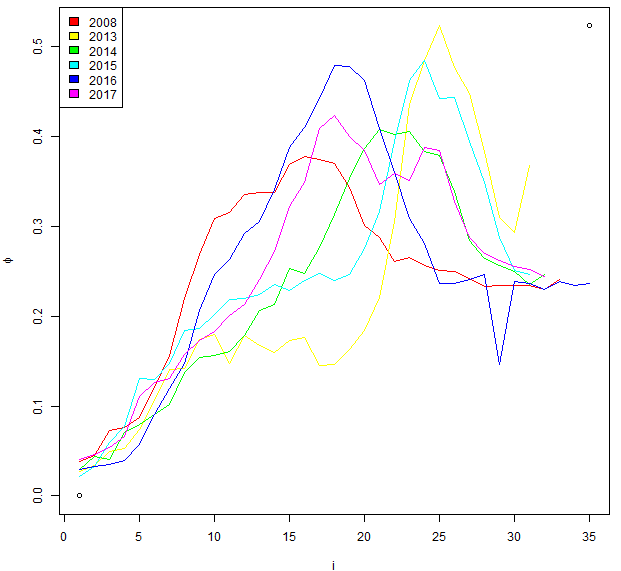
\includegraphics[width=5.5in]{PhiParAnnee.png}
    \caption{$\phi_i$ pour chaque ann\'ee.}
\end{figure}

On voit qu'aux environs de sept semaines avant la fin de l'\'epid\'emie les courbes semblent
graviter autour de $\phi = 0.15$. On utilise la fonction \texttt{cut} dans R\cite{R} pour cr\'eer des
intervalles dans lesquels on va trouver celui dont l'\'ecart-type du nombre de semaines pour chaque
saison avant la fin de l'\'epid\'emie est minimal. Nous avons test\'e toutes les valeurs de $\alpha$
allant de 0.10 \`a 0.90 en bond de 0.01 et le nombre d'intervalles entre 4 et 12 pour trouver
$\alpha = 0.77$ avec notre $\phi$ id\'eal $\psi = 0.148$.  Le nombre de semaines pr\'edit avant la
fin de l'\'epid\'emie pour $\phi_i = \psi$ est de 7.75 semaines avec un \'ecart-type de 0.71
semaine.

Sachant que notre \'equation doit correctement pr\'edire qu'en $\phi_i \approx 0$ l'\'epid\'emie est
fonctionnellement termin\'ee et qu'on estime qu'en $\phi_i = \psi$ il reste environ 7.75 semaines
avant la fin de l'\'epid\'emie, nous obtenons l'\'equation lin\'eaire suivante:
\[ S_i = \frac{\phi_i}\psi 7.75 \]
\`A l'aide de cette formule nous pouvons tracer le graphe de l'estimation du nombre de semaines
restantes avant la fin de l'\'epid\'emie, et ce, pour chaque ann\'ee.

\begin{figure}[h]
    \centering
    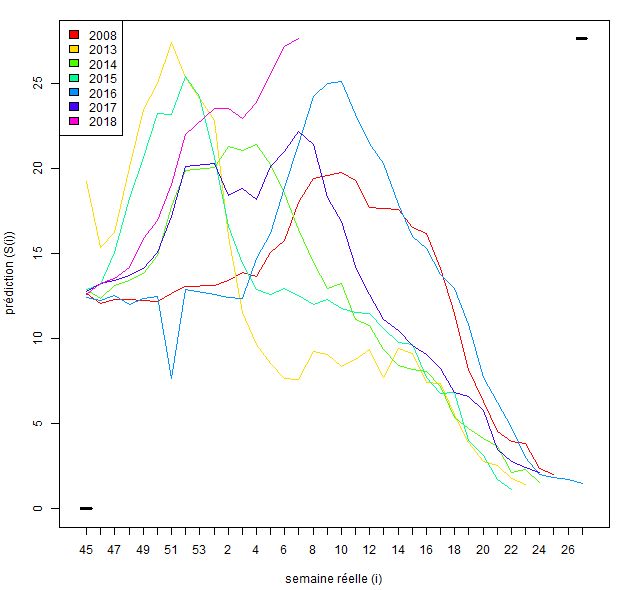
\includegraphics[width=5.5in]{PredictionParAnnee.png}
    \caption{$S_i$ pour chaque ann\'ee.}
\end{figure}

On voit bien que le mod\`ele ne produit pas de donn\'ees utiles avant que l'\'epid\'emie ait atteint
son paroxysme. Toutefois, le nombre de semaines pr\'edit en tout point ult\'erieur \`a ce dernier,
pour chaque ann\'ee, ne s'\'eloigne pas trop de la r\'ealit\'e. Nous avons calcul\'e que l'\'ecart
moyen \`a notre pr\'ediction du nombre r\'eel de semaines \`a la fin de l'\'epid\'emie, pour chaque
semaine pass\'ee le paroxysme, est d'environ 19\% pour les ann\'ees pass\'ees. D'autre part, nous
avons essay\'e de multiples valeurs de $\alpha$ et observ\'e que les r\'esultats varient peu.

Pour am\'eliorer nos deux param\`etres, nous pourrions aller chercher des donn\'ees similaires dans
les autres parties du monde, en particulier dans l'h\'emisph\`ere sud o\`u la grippe est aussi
saisonni\`ere. Nous pourrions aussi essayer de pond\'erer les souches A et B ind\'ependamment avec
des param\`etres $\alpha$ et $\beta$.

Une fois les constantes d\'etermin\'ees, le mod\`ele est simple \`a appliquer aux donn\'es
courantes; il suffit d'\'evaluer la fonction avec les tests d'une semaine donn\'ee. Un dirigeant
peut donc prendre des d\'ecisions utiles sachant qu'elles seront d'autant plus pertinentes que le
paroxysme sera pass\'e. Le mod\`ele est extensible au nombre de souches pr\'esentes au sein d'une
population quelconque. Il semble que les donn\'ees utilis\'ees par notre mod\`ele soient disponibles
dans un grand nombre de r\'egions du monde. Nous avons r\'epertori\'e le reste du
Canada\cite{InfluenzaCAN}, les \'Etats-Unis\cite{InfluenzaUSA} ainsi que la France\cite{InfluenzaFRA}
r\'ecoltant ce type de donn\'ees. Un pays avec un syst\`eme de sant\'e utilisateur-payeur comme les
\'Etats-Unis peut utiliser notre mod\`ele sans probl\`eme puisqu'il ne n\'ecessite pas de donn\'ees
absolues mais bien des proportions.

Les pr\'edictions du mod\`ele sont probablement moins utiles pour les r\'egions \'equatoriales l\`a
o\`u la grippe n'est pas saisonni\`ere. Par ailleurs, le mod\`ele est incapable de produire des
pr\'edictions fiables lorsque l'\'epid\'emie est encore aig\"ue. Apr\`es avoir exerc\'e le mod\`ele
sur les diverses ann\'ees, on voit bien qu'il y a des donn\'ees aberrantes, en particulier la saison
\'epid\'emique de 2013 semble avoir perdur\'ee tr\`es longtemps.

Nous aimerions pouvoir investir d'avantage de temps et d\'eterminer s'il est possible de cr\'eer
un mod\`ele plus puissant qui s\'epare la pond\'eration entre les souches et pond\`ere les
estimateurs de fa\c con progressive. Par exemple, on pourrait calibrer nos param\`etres en fonction
d'une pond\'eration in\'egale entre les diverses souches en relation avec le temps depuis le d\'ebut
de chacune. On obtiendrait ainsi une \'equation \`a plusieurs variables et param\`etres.

\section{Conclusion}
Nous pensons que le mod\`ele obtenu permet d'obtenir une pr\'ediction raisonnable du nombre de
semaines avant que l'\'epid\'emie soit fonctionnellement termin\'ee (moins de 1\% de d\'etection).
Compte tenu de l'impact socio-\'economique important de ce virus, nous croyons que cette derni\`ere
mesure est appropri\'ee pour estimer le degr\'e de dangerosit\'e de l'\'epid\'emie d'influenza.

L'utilisateur doit \^etre conscient que la pr\'ediction est peu fiable lorsque l'\'epid\'emie est
aig\"ue. En particulier, la saison 2018 bat son plein et donc est tout \`a fait dangereuse. Nous ne
croyons toutefois pas qu'elle durera encore 27 semaines tel que notre mod\`ele l'indique.
\clearpage

\begin{thebibliography}{9}
    \bibitem{R} \href{https://www.r-project.org/}{The R Project for Statistical Computing}
    \bibitem{Deces} \href{http://www.who.int/mediacentre/news/releases/2017/seasonal-flu/en/}{Death statistics}
    \bibitem{Impact} \href{https://en.wikipedia.org/wiki/Flu\_season\#Cost}{Cost of the Flu season}
    \bibitem{InfluenzaQC} \href{https://www.inspq.qc.ca/influenza}{Surveillance de l'influenza (QC)}
    \bibitem{InfluenzaCAN} \href{https://www.canada.ca/fr/sante-publique/services/maladies/grippe-influenza/surveillance-influenza/rapports-hebdomadaires-influenza.html}{Surveillance de l'influenza (CAN)}
    \bibitem{InfluenzaUSA} \href{https://www.cdc.gov/flu/weekly/}{Surveillance de l'influenza (USA)}
    \bibitem{InfluenzaFRA} \href{http://invs.santepubliquefrance.fr/Dossiers-thematiques/Maladies-infectieuses/Maladies-a-prevention-vaccinale/Grippe/Grippe-generalites/Donnees-de-surveillance}{Surveillance de l'influenza (FRA)}
\end{thebibliography}
\end{document}
